\documentclass{article}
\usepackage{amsmath}
\usepackage{graphicx}
\usepackage{wrapfig}
\usepackage[margin=1in]{geometry}
\usepackage[square,numbers]{natbib}
\bibliographystyle{unsrt}

\title{Adaptive EdgeAI in an intelligent Scientific Information Maketplace}
\author{Ryan Coffee}

\begin{document}

\maketitle

\paragraph{Abstract:} %The advent of very high frame-rate sensors as needed for the upcoming ultra-high duty cycle user facilities in the Department of Energy research portfolio necessitates a fundamental shift in how experimental data is recorded and stored.
A continued exponential increase in value from scientific experiments can only endure the impending end of Moore's scaling if we reinvent how experimental data is recorded, stored, and compared with theory.
We must develop an intelligent data pipeline that is reconfigurable, robust, and reconstructable that incorporates machine learning and enables autonomous real-time decision making.
The reinvention of such a processing chain should not only produce unique data identifiers, but should incentivize open sharing in a market place whereby data producers receive credit for data generation that is commensurate with the impact afforded to data consumers via publication and technology transfer.

\section{Motivation}
\begin{wrapfigure}[33]{r}{.5\linewidth}
	\centerline{ 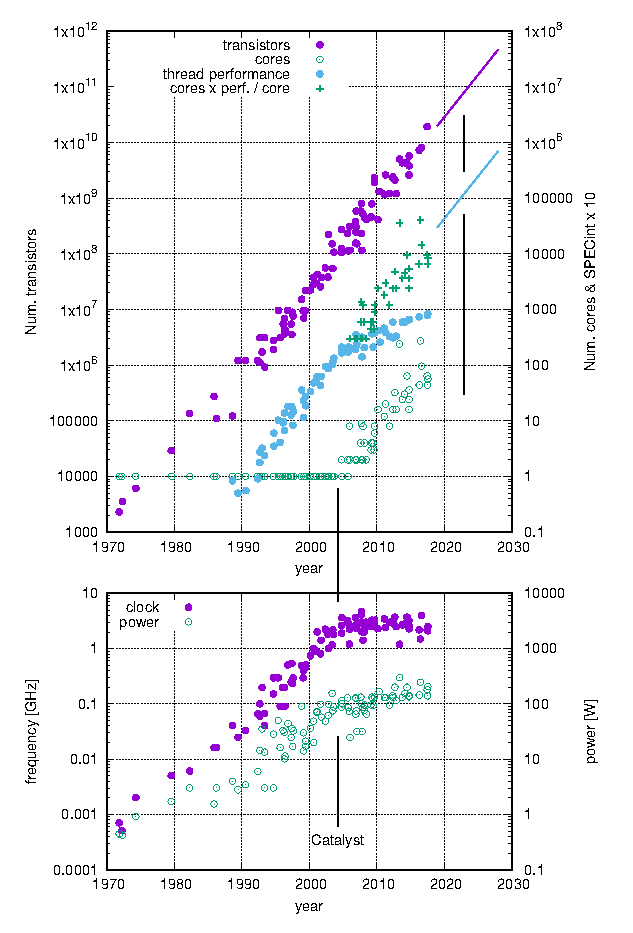
\includegraphics[clip,trim={-2cm -2cm 1.5cm 1.5cm},width=\linewidth]{plotting_technology.eps} }
	\caption{
		\label{fig::technology} 
		Data adapted from Ref.~\cite{MicroprocessorTrendData}. 
	}
\end{wrapfigure}

\subsection{Information not data}
\paragraph{Exponential advancement}
Scientific advancement, like all human technological advancement \cite{Kurzweil}, progresses with exponential rapidity.

However, raw data rates are also increasing at an exponential rate and therefore are now growing to data velocities (TB/s) that exceed network and storage capacity.  
This challenge is shared with the private sector, notably, AI assisted agriculture whereby extant hyperspectaral imaging technology can not be appropriately leveraged simply owing to its excessive data velocity.

\paragraph{Impending phase transition}
In the upper panel, the utility of increasing compute enabled by increasing transistor density has value matched by the compensation of the roll off of thread performance by increasing the number of concurrent threads.
The roll off in thread performance is temporally correlated with the GHz limit in clock frequency as noted in the text.

The thermal conductivity of liquid water is on the order of $k \sim 7 \mbox{mW} \mbox{cm}^{-1} \mbox{K}^{-1}$.
The conductance of heat from the chip is governed by $q = k \delta T / \delta x \sim \mbox{mW} \mbox{cm}^{-2}$ assuming $\delta T \simeq 50 \mbox{K}$ and $\delta x \simeq 0.1 \mbox{cm}$ is about 3.5 $\mbox{W} \mbox{cm}^{-2}$.
For a heatsink of about $2\mbox{cm}\times2\mbox{cm}$ with 2 cm tall vanes separated by 1 mm gives a total surface area of about $80 \mbox{cm}^{2}$ and thus corresponds to a thermal dissipation capacity of 280 W.
We note that the in the bottom panel of Fig.~\ref{fig::technology} we see that the power of the processors looks to be approaching a few hundred Watt assymptote.
Likewise, the speed of light is 30 cm/ns such that the typical chip scale of 3 cm corresponds to one wavelength of 10 GHz light, and so it is no surprise that our clock rates have run into a limit in the vicinity of few GHz.
These physical limitations have motivated a the shift away from thread performance with faster clocks in favor of multi-threaded processing that can better leverage the utility of the increased transistor density.
In the next decade, we will likely see the transistor size encroach on a qunatum mechanical limit of tens of atoms wide transistors, and this limit will again motivate a redesign of some other part of the computing story.
We purport that the redesign will be in how we consider the value of data versus information.

Physical limitations motivate us to rethink how we extract value from computing.  
We are opening the data volume flood but at a time when we wil lbe hitting a physical wall in computing, so now is an opportune moment to rethink how we extract value from recorded data.

We predict another catalyzing event in the first half of the 2020s.
Sometime early in this decade the size of transistors will approach the a quantum mechanical scale of tens of atoms along a dimension.
As observed in the mid-2000s, the then catalyzing limit of clock frequencies approaching the wavelength of light comparable to the physical dimension of the chip and the power dissipation comparable to the capacity of cooling systems, we saw a move toward parallel architectures. 
This transition is very nicely coincident in time with the physical clock and power limitations but we see the innovation step toward multi-threading allows the continued exponential growth of compute utilization by now scaling the physics limited per-thread efficiency by parallel algorthm design.
By scaling the per-thread efficiency by the numer of cores (blue triangles) in Fig.~\ref{fig::technology}, we see that parallelization allowed computing value to keep pace with the still exponential transistor growth in spite of the clock and power physical limitations.

We predict that a similar catalyzing physical limitation will arrive in the early 2020s as the transistor dimension encroaches on the atomic limit.
When this dimension is reduced to the 1 nm scale, the quantum mechanical properties of groups of tens of atoms will begin to dominate the function of transistors.
Barring a wholescale conversion to quantum computing, an alternative classical computing innovation, and one particularly important to the future of machine learning, could be a shift in how we view data versus information.

\paragraph{Data liability}
But the Department of Energy is not alone in its quandry regarding ever increasing data volume and velocity.
In a recent conversation with a representative of the agriculture industry, the use of hyperspectral imaging would be revolutionary, but the data volume produced is prohibitively impractical for real-world industrial agricultural application.
The information contained in the 3 dimensions of 2 spatial and 1 spectral could deliver exquisite predictive power, except that such sensors run in remote areas typically in areal drones and thus have limited local storage and network capacity.
As with the high speed sensors being developed by the Department of Energy that are expected to keep abreast of the TBs per second potential data rates, we face the increasingly well understood liability of excessive data. 
Novel event based camera technology is arising both within DOE R\&D programs and in the commercial sector \cite{Prophesee}.  
Such technology will work well to capture relevant changing visual fields elements while suppressing the storage of still backround information, but in many applications in science, the backgrounds that should be suppressed are themselves vayring in time, and therefore a domain specific foreground/background identification must be implemented.

\paragraph{Adaptive data-to-information mapping}
For such experiment specific cases, we seek a computing solution that allows for user costomizable logic, be it conventional algortihm or custom machine learned inference models.
In either case, the bespoke logic design will likely require adaptation to the existing computational environment, and as we have already begun to see with FPGAs, some architectures are better suited to GPUs than they are for FPGAs, and vice versa.
One fairly common trend observed is that the GPU is better adept at dynamically changing the model over the course of hours or days, while the FPGA is a robust and high throughput data pipeline machine, but is significantly more fragile to even well compartmentalized modification.
We expect therefore that FPGAs will likely collect in the early 


The upcoming very high frame-rate sensors and the correspondingly ultra-high duty cycle user facilities in the Department of Energy research portfolio requires use of low-latency and very high through put data processing engines that typically have very different compute constraints than conventional cloud-based machine learning.

We propose a shift to processing information at or very near to the point of production, ideally in the experimental sensors themselves, that provides orders of magnitude in data compression while preserving both validation and forensic reconstruction of decision chains.

\paragraph{Data Flow at the Edge}
\begin{figure}
	\centerline{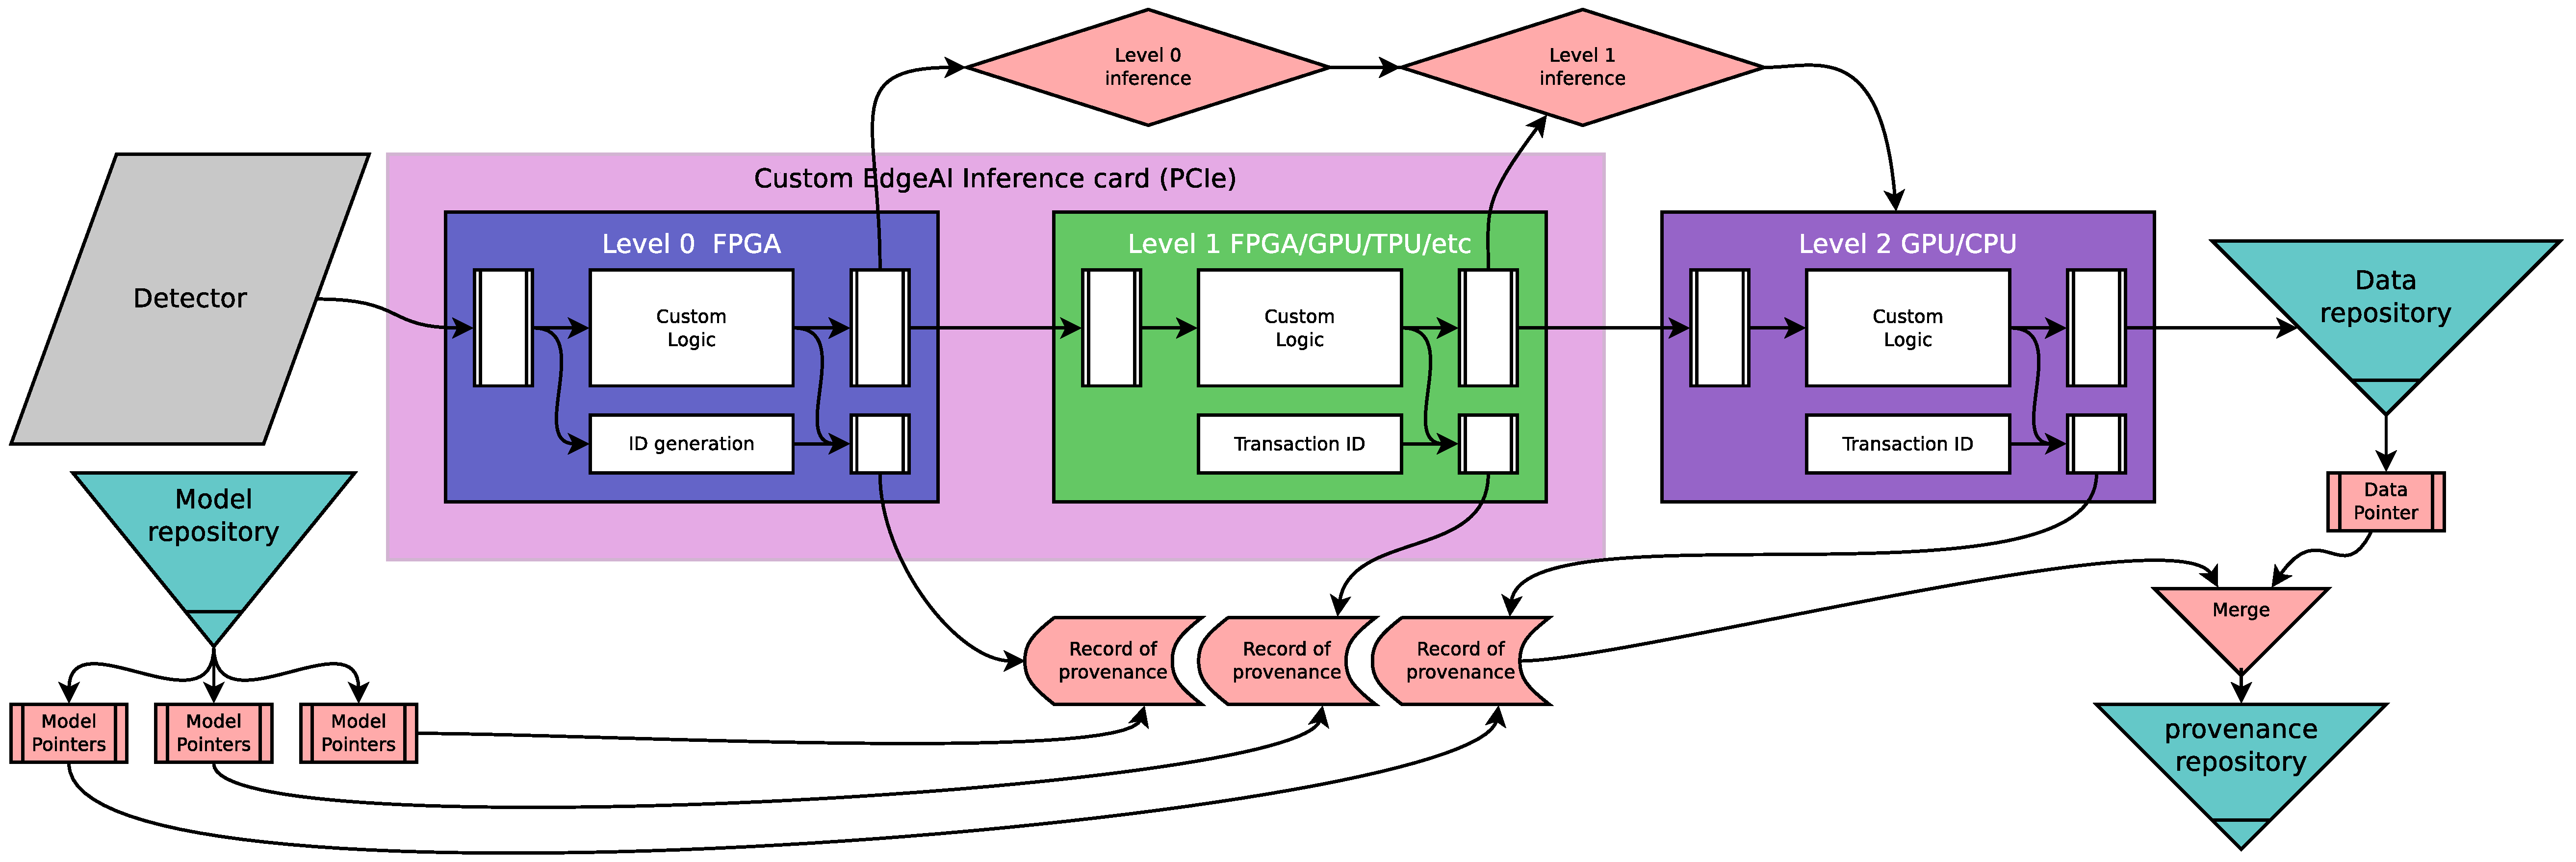
\includegraphics[clip,width=\linewidth]{EdgeFlow.eps}}
	\caption{
		\label{fig::EdgeFlow}
		Schematic of information flow through heterogeneous hardware with ID generation and provenance tracking.
		}
\end{figure}

An interoperable stack with fundamental coupling between algorithm and data individuals would allow for multiple data pipelines, some very low latency for making feedback control decisions, and others that are higher fidelity though lower throughput that provide validation and testing.  Furthermore, this is critical in a sensor ecosystem whereby the sensor reporting duty cycles may have vastly different timescales. 
This is not unique to DOE facilities like the LCLS-II where come sensors will report at the 1MFps machine rate and others at a much slower e.g. pre-scaled 100Hz "validation" rate.  
In the agriculture industry, aereal drones can provide hourly hyperspectral imaging data while soil testing likely occurs at most daily or monthly, thus also a multiple duty cycle sensor reporting rate that needs be fused.

Provenance must be fundamentally included together with the data in particular as it is required for data fusion, and uplimately for forensic reconstruction in our common case of very high price of being wrong in autonomous inference.




\subsection{Adaptive EdgeAI}
\paragraph{Adaptive algorithms}
Data curation must be fundamentally integrated into the design of the data acquisition.  This is a tremendous challenge in the context of DOE user facilities where the data transfomraion chain, the algorithm/data transaction chain, will make step changes each experiment cycle, every week at every beamiline will be a new data representaiton algorithm which will need to accommodate user and domain specific algorithms.
This domain specificity lends better to a model of heterogeneous edge hardware whereby the data and algorithm identifiers are built into a transaction log or ledger while the specific algorithm is flashed to a user accessible logic region.
In FPGAs for instance, there can be IPcores that are hidden from user access.  These cores allow the Data Stack infrastrucure.  The user logic cores then serve the domain specific, potentially user developed, data transfomration logic and algorithm.

\paragraph{Heterogeneous Hardware}
Autonomous data routing and adaptive data mapping algorithms that are triggered by single event measurements \cite{Lutman2016,Wolfi2017_review,Hartmann2018} would allow for multiple targeted data sets to be recorded simultaneously.  
For instance, in the case of SASE x-ray pulses, one user group may desire single attosecond pulse \cite{Cryan2016_impulsive} result while another group would prefer two-pulse x-ray pump-probe conditions \cite{Hartmann2018}.  
Yet another group might prefer the stochastic spectral and temporal fluctuations \cite{Feurer2018,IanRobinson2018,Driver2019_spooktroscopy} that the other two groups would likely veto.  
An autonomous data routing mechanism for on-the-fly adaptive data treatment could therefore use three specific analysis chains that would individually treat the incoming events appropriately for the targeted scientific interpretaiton.
The upstream so-called ``data-router'' \cite{Audrey} would be implimented in the earliest layers in the data pipeline, allowing for dynamic routing through one of the three static analysis chains which themselves would likely be implimented in acceleration hardware either on-board or via PCIe bus in the recording computer node.
%Example is using an x-ray attosecond double pulse experiment that quietly records spooktroscopy data with a forked data path. The producer of the spooltroscopy data then gets credit for his/her background production of that data even though that wasn’t the original goal of the experiment.

\paragraph{Scientific Integrity versus the AI Black Box}
In this scenario, however, each data acquisition event would potentially incure a chain of analysis manipulations or flow through different inference models or compression encodings.
This chain would be unique to the target scientific domain with each sensor event serving as the initial unique seed for the respective analytic transaction chain.
By fundamentally encoding the event seeded routing decision chain, one could not only produce a unique data identifier that can be used to later to identify valuable with original data, but also it allows for the domain-specific forensic reconstruction of the analysis pipeline, assuming the transaction record also provides pointers to the inference models that were active in the pipeline.
Such a task is likely prohibitively cumbersome unless we avoid precise network syncronization by using the analytic hardware itself to both flow the data and to simultaneously produce the transaction record.

\subsection{Scientific Information Marketplace}
Models that map raw data input to lower dimensional information. 
\paragraph{Current challenges}
Conventional data warehouses collect and organize only the data that is generated in premisis or within the tight knit collaborative group.
This is the typical case for DOE facilities that generate enormous high velocity data, there is typically an on premesis data storage facility that houses all raw data generated by the facility and allow temporary user storage for auxillary and or augmentation data used for analysis and interpretation, e.g. intermediate analysis stages and code repositories.
More common than on-prem code repositories is the changelog of code evolution that is tracked via git, svn or other code repositories.
Unfortunately, such code repositories are not tightly coupled to the data these codes were used to manipulate.

\paragraph{The information marketplace}
The Data Stack is like a supply chain, each analysis step or ML model application is a data manipulation or mapping that constitutes a transaction between the algorithm unit and the data unit.
Each transacting party should retain a ledger of the applied transactions with an identification marker unique to the algortimn or data unit.


The Data Stack compiles disparate data shards or individuals as potentially multi-modal data collections, with the associated mapping algortihms will make for a more fundamentally integrated data fusion infrastructure.

\paragraph{Embargoes and Retention}

\paragraph{Sharing is Caring, or share what you don't care}

One approach is Government initiative toward altruistic data sharing, however this is often at odds with individual motivations for e.g. tenure, professional recognition, attracting graduate students, procuring grant funding and also appropriately assigning credit to government funded research facilities for their roles in data prduction.  Typically the scientific credit is only delivered to the data consumer, however the providers (DOE labs) lie at the foundation of the data economy.
If there is a measureable and tracable value metric, then the entire data production chain, from accelerator operation and construction to detector creation and development all the way to new technologies transferred to comercial sector would recieve the due credit.

The example we like is that a light weight classification network running in a diagnostic detector could signal single or double shots and veto multiple SASE spike events.
A more inventive approach would be that users would be prompted with a query window if they would allow the quiet collection of the veto data for use in community open access data repository that would be free of access restriction embargo.
Such a repository could then serve as algorithm development research and ultimately help improve the Edge models used in future experiments.
When such data from the community repository is used for improvements and or publication, then there will be a note of credit ascribed to the generating experiment as the data producer.
Such credits could then serve as metrics for both the facility, the detector, the FEL operation mode, and even the experimenter his or herself, increasing likelihood for subsequent beamtimes for instance.
Such incentives would then encourage users not only to open the ``veto'' data to un-embargoed repositories, but it would also create a value for being a data producer rather than exclusively assigning academic credit for data developers and financial gain for data consumers as is the current paradigm.

Researchers physically cannot incorporate the developing methods at the rate of ideation, but the future of AI assisted scientific discovery would allow for the near real time implimentation of novel new methods if not directly at experiemtnal execution, then shortly thereafrter based on known data and recoverable raw data.

\paragraph{The data supply chain}
The second missing step is that the data producers, owners, and curators all work together.  This we can motivate if the data identifiers themselves can carry a representaiton of value, a value that get incremented whenever a data individual or algorithm unit is used or referenced in publication and research value metrics.
This motivation ideally support something of a data economy such that it will self sustain as a community economic system.  But this econmomy can't be based on raw data, that would be fragile to hyperinflation, but if there is real measurable and tracable value to the data and respective algorithms, then we move into an information economy whereby information we mean the valuable combination of data nad algortihm.

Adapted from Ref.~\cite{Elbaz2012} we follow an example of a supply-chain like data stack: % http://blog.factual.com/how-the-data-stack-can-organize-your-data-science-program
\begin{itemize}
\item Providers, these are the instruments and sensors that report state during data acquisition as well as the scientific detectors themselves (those who have data that may be able to help create a valuable data set.)
\item Curators, these are likely the instrument scientists and user consortia who agree upon dommain specific representations and shareable labels. (those who collect data from providers, use technology and other means to create valuable datasets, and then provide it to developers and consumers.)
\item Developers, these are the individual PIs at labs and universities who combine the curated data into scientifically meaningful models in their expertise domains. (those who use the data from curators and providers to create or enhance products.)
\item Consumers, likely this is the private sector companies who wil leverage the scientific developments to promote commercially viable technology transfer paths. (those who make use of the data directly or through products.)
\end{itemize}


In a data economy, one could imagine not only a single lab economy, but also an inter-lab and ultimately an international data economy.



\section{Scope}

\subsection{Algorithm Development}
\paragraph{Facility based sharp inspirational examples}
\paragraph{Hardware dependent architecture considerations}
Depending on the data mappings, a suggestion engine could recommend what background transformation chains would a) fit the hardware, and b) maximize the likelihood of background data relevance for the broader external community.

\paragraph{Developing a palette of hardware}
The layer with the highest connectivity will likely be the longest latency layer in a given neural network, therefore one would design early data routing decisions at the highest throughput level to determine the downstream routing for a given event.  

\subsection{Transaction record}
\paragraph{ID generation at point of production}
\paragraph{Model encoding into transaction record}
\paragraph{Forensic reconstruction via pointers to original data}
\begin{itemize}
\item Unique data identifiers
\item Ledger of training samples used to produce models
\item Ledger of model chains in decision chain, tied to the data
\end{itemize}
\paragraph{SmartID for tracking data value that informs embargo and retention decisions}

\section{Schedule}

\section{Cost -- 650K\$/year $\times$ 3 years}
\paragraph{Algorithm Development and Heterogeneous Hardware} 0.3 FTE PI .3*250K, 1FTE SLAC RA 180K, 1 Grad student 150K, sub-contract with UNUM @ 120K per year
\paragraph{SLAC FPGA work} 0.25 FTE TID .25*400K
\paragraph{Transaction Record} 0.2 FTE PI 60K, 0.4 Staff 120K, Sub-contract with Altered Silicon @ 120K per year
\paragraph{Hardware} 50K edge computing year 1, 50K custom PCIe board for MCP signal ingest year 2.  50K second custom PCIe board for imaging CXP12 ingest year 2.











\pagebreak
\section{Notes}




















"Because we have an intuitive understanding of data, often we don’t ask important questions. We
know what data is, how it can be stored, how to move it, how to analyze it, and in a sense, we
think we understand the nature of data.
But a closer look at the world of data shows that there is no Moore’s Law in effect. More data
just means more data. In many cases data is a liability. More data means more costs for storage,
for governance and having too much unorganized data may make it more difficult to find what
you need. In other words more data can mean less value." -- Dan Woods \cite{Woods2013}
%"How To Create A Moore's Law For Data" Forbes Dec 12 2013, https://www.forbes.com/sites/danwoods/2013/12/12/how-to-create-a-moores-law-for-data/#7051ed4f44ca

"To make a Moore’s Law for data, we also need two layers, a data stack and a data economy layer. If both of these layers were as mature as the hardware and software industries, more data would
mean more value." -- Dan Woods \cite{Woods2013} %"How To Create A Moore's Law For Data" Forbes Dec 12 2013, https://www.forbes.com/sites/danwoods/2013/12/12/how-to-create-a-moores-law-for-data/#7051ed4f44ca

\subsection{The Data Stack}

"The data stack defines all the capabilities needed to connect to data, collect it, clean it, and join it together into a form that makes sense.
Then the data stack describes capabilities for delivering that data to those who use it in multiple
ways, through subscriptions or through APIs." -- Dan Woods "How To Create A Moore's Law For Data" Forbes Dec 12 2013, \cite{Woods2013} %https://www.forbes.com/sites/danwoods/2013/12/12/how-to-create-a-moores-law-for-data/#7051ed4f44ca


"Data stacks assume that data must be curated and maintained, in other words data is both
an asset and a liability. Often, the fact that a data set is actually a liability is ignored in
much data processing. In data stacks, the responsibility for curation is addressed as part
the initial design." -- Dan Woods "How To Create A Moore's Law For Data" Forbes Dec 12 2013, \cite{Woods2013} %https://www.forbes.com/sites/danwoods/2013/12/12/how-to-create-a-moores-law-for-data/#7051ed4f44ca


Some counter examples are the Materials Data Base, Observational astronomy, HEP.  Still, these counter examples benefit from a community consensus for data structure and 

%Look up Why Building a Distributed Supply Chain is More Important than Big Data -- http://www.forbes.com/sites/danwoods/2013/06/27/why-building-a-distributed-data-supply-chain-is-more-important-than-big-data/



%% look up Factual %% to see what they have/are building.



"One huge barrier Elbaz points out is the assumption of altruism that seems to motivate many
efforts at sharing data, especially projects that fall under the open data umbrella. When
organizations consider sharing data, they often incorrectly assume that they must just give the
data away and hope that some benefit accrues to someone. Government initiative have resulted
many victories using this model. But organizations are sitting on massive troves of data that
won’t be shared unless there is a fair trade."




\bibliography{whitepaper.bib}

\end{document}
